\documentclass[10pt]{article}
\usepackage[T1]{fontenc}
\usepackage[utf8]{inputenc}
\usepackage[a4paper,margin=1cm]{geometry}
\usepackage[colorlinks=true,linkcolor=black,urlcolor=black]{hyperref}
\usepackage{titlesec}
\usepackage{enumitem}
\usepackage{multicol}
\usepackage{microtype}
\usepackage{tabularx}
\usepackage{graphicx} % for photo
\setlength{\emergencystretch}{3em}
\pagenumbering{gobble}
\setlength{\parindent}{0pt}
\setlength{\parskip}{1pt}
\linespread{0.9}
\titleformat{\section}{\large\bfseries}{}{0pt}{}
\titlespacing*{\section}{0pt}{3pt}{1pt}
\setlist[itemize]{leftmargin=10pt,itemsep=-1pt,topsep=0pt,parsep=0pt,partopsep=0pt}

\begin{document}

\noindent
\begin{tabularx}{\textwidth}{X c}
{\LARGE \textbf{Arman Shirzad}}\\
Cottbus, Germany \quad \href{mailto:shirzarm@b-tu.de}{shirzarm@b-tu.de} \quad {+49 157 5669 3804}
&
\raisebox{-0.5\height}{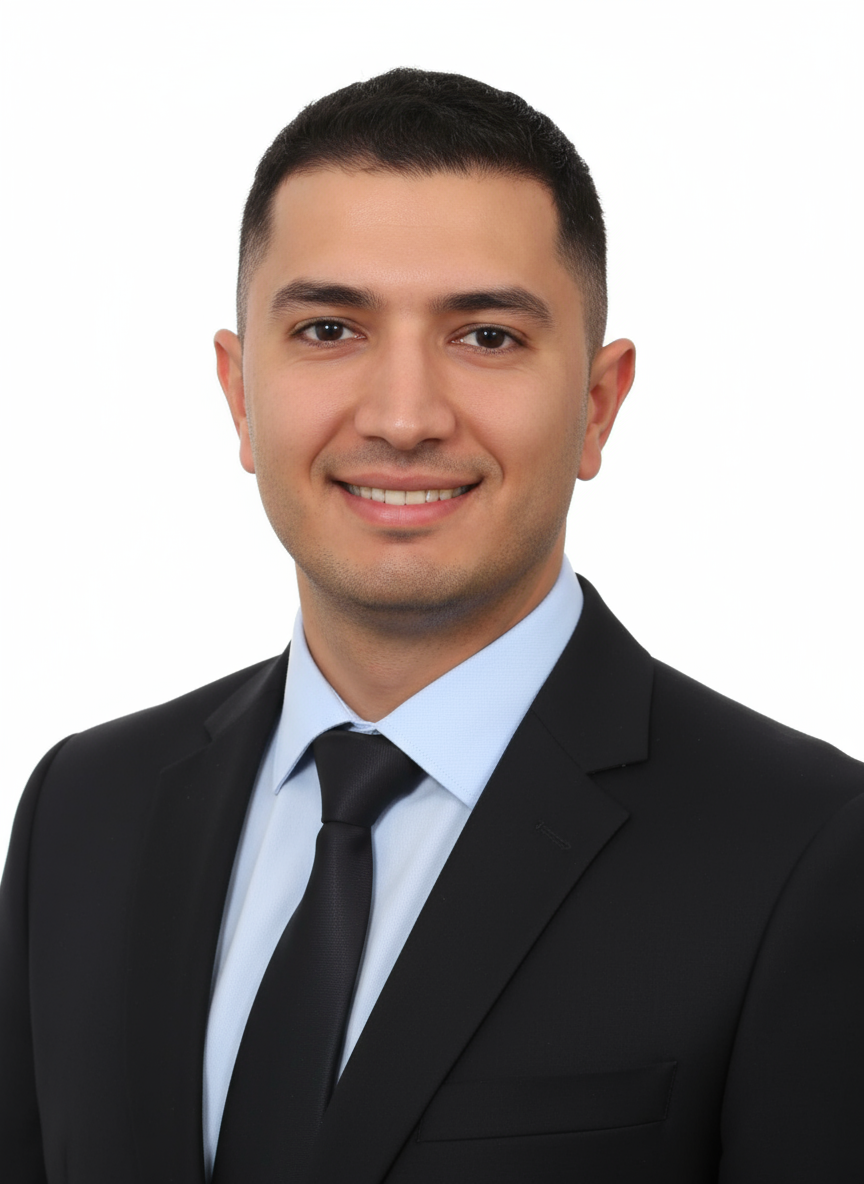
\includegraphics[width=3cm,height=4cm]{presidency photo.png}}
\end{tabularx}

\section*{Kurzprofil}
Masterstudent der Künstlichen Intelligenz (BTU). Starker Software-Engineering-Fokus mit C\#, Python, robusten Backends, automatisierten Tests und Releases, Cloud und DevOps. Übersetzt komplexe Technik präzise für technische und nicht-technische Stakeholder. \textbf{Auf KI spezialisierter Softwareentwickler mit starker Backend- und DevOps-Grundlage.}

\section*{Berufserfahrung}
\textbf{Software Engineer} \quad Refah Bank, Tehran \hfill 08/2022 bis 03/2025\\[-1pt]
\begin{itemize}
  \item Elektronische Stempelplattform auf ASP.NET Core (CQRS, MediatR, EF Core, SQL Server), Messaging mit RabbitMQ/NServiceBus, Auth mit IdentityServer, API-Gateway.\textbf{\(\sim 10{,}000\) Requests/Tag, > 2\,Mio. Stempel, MTTR um 40\,\% gesenkt}.
  \item Legacy-Monolith auf C\# ASP.NET Core APIs modernisiert (Clean Architecture, automatisierte Tests, Docker, CI/CD). \textbf{Ausfallzeit um 30\,\% reduziert}.
  \item Neobank-Schnittstellen für \(\sim 200{,}000\) Nutzer integriert. Resilienz durch Retries, Circuit Breaker und Versionierung; Skalierung im Team umgesetzt.
  \item Architektur- und Performance-Tuning über 15+ Services und externe Integrationen.
\end{itemize}

\textbf{Software Developer} \quad MAPSA Technology Center, Tehran \hfill 03/2021 bis 07/2022\\[-1pt]
\begin{itemize}
  \item WPF-/MVVM-Tool für KPI-Analysen in der Ölbohrung entwickelt; asynchrone Pipelines optimiert, \textbf{Berichtszeiten um 40\,\% verkürzt}.
  \item Git-Workflows eingeführt und Teams über 3 Monate geschult; Migration von TFS zu Git begleitet.
\end{itemize}

\textbf{Full Stack Software Engineer} \quad Freelance, Remote \hfill 08/2020 bis heute \\[-1pt]
\begin{itemize}
  \item 12 kundenspezifische APIs für SaaS/E-Commerce geliefert; \textbf{p99 Latenz < 120\,ms}.
  \item Bots für Telegram, Discord, WhatsApp; manuellen Posting-Aufwand deutlich reduziert.
  \item Docker und GitHub Actions für CI/CD; Releases von Stunden auf Minuten verkürzt, Zero-Downtime-Deployments.
  \item 5 KMU-Workloads mit Terraform auf Google Cloud migriert; \textbf{Kosten \(\sim 30\,\%\) niedriger}, tägliche Kostendashboards.
\end{itemize}

\section*{Projekte}
\textbf{Elektronische Stempelplattform} \quad Skalierung und Betrieb bei hoher Last.\\
\textbf{NASA Exoplanet Detection Platform} \quad Leitung eines internationalen 5-köpfigen Teams; End-to-End-Pipeline für Datenaufbereitung, Modellierung und Deployment als Lead Engineer.\\
\textbf{GCP Cloud Resource Analytics} \quad Serverlose FastAPI Ansicht mit Terraform, Asset und Kostenreports.\\
\textbf{Telegram Gruppen Audit Bot} \quad Google App Engine, Task Queue, kleines Admin Interface.\\
\textbf{Social Media Content Automation} \quad Orchestrierung von Plattform-APIs, Scheduling, Content-Generierung und Analytics-Pipelines (Automatisierung, Monitoring, Reporting).\\
\textbf{qrRobust Scanner} \quad Ursprünglich als persönliches Projekt gestartet, anschließend zu einem etablierten Open-Source-Tool skaliert.\\

\section*{Ausbildung}
\textbf{Master of Science in Artificial Intelligence} \quad BTU Brandenburg \hfill 03/2025 bis heute\\
\textbf{Bachelor of Engineering in Computer Software Engineering} \quad University of Science and Culture \hfill 09/2016 bis 10/2020

\section*{Kenntnisse und Fähigkeiten}
\begin{multicols}{3}
\begin{itemize}
  \item Programming \& Backend: C\#, Python, SQL, JavaScript/TypeScript, Bash, REST, GraphQL
  \item Frameworks: ASP.NET Core, EF Core, FastAPI, WPF/MVVM
  \item Architecture: Clean Architecture, DDD, CQRS, API Gateway
  \item Data \& Search: SQL Server, PostgreSQL, MySQL, MongoDB, Elasticsearch
  \item Vector Stores: Qdrant, Milvus, Pinecone
  \item Messaging \& Cache: RabbitMQ, Redis
  \item AI/LLM: RAG, LangChain, Transformers, LoRA/QLoRA, Prompt Design
  \item Data Tools: NumPy, pandas, SciPy, Matplotlib
  \item Cloud \& DevOps: Google Cloud (App Engine, Cloud Run, Cloud Build, Secret Manager), cost dashboards
  \item Automation \& IaC: Docker, Terraform (environments, workspaces, policies)
  \item Orchestration: Kubernetes, Helm
  \item CI/CD: GitHub Actions, Azure DevOps, trunk based development, release management
  \item Version Control: Git/GitHub, TFS, rebase, squash, cherry pick, GitFlow
  
  \item Security \& APIs: IdentityServer, OAuth~2.0, OpenID Connect, JWT, rate limiting, versioning
  \item Testing \& Quality: unit/integration (xUnit, NUnit, pytest), BDD (SpecFlow/Gherkin), Selenium/Playwright, load testing, Jest/RTL
  \item Frontend: HTML, CSS, Bootstrap, Tailwind, React (fundamentals), Redux/Zustand
  \item Build \& Tools: dotnet CLI, pip, poetry, make, nox
  \item Product \& Delivery: MVP scoping, requirements analysis, SRS/BRD, backlog grooming, Scrum/Kanban, code review, documentation
  \item Collaboration: Azure Boards, Jira, Figma, Visio, UML
  \item Research \& Writing: LaTeX/Overleaf, literature review, bibliometric study
\end{itemize}
\end{multicols}

\section*{Publikationen}
\begin{itemize}
  \item A Bibliometric Analysis of Quantum Machine Learning Research. \emph{Journal of Science and Technology Libraries}, 2024. \href{https://doi.org/10.1080/0194262X.2023.2292049}{DOI}
  \item Text Independent Speaker Recognition  A Novel Deep Learning Approach. \emph{CoDIT}, 2024. \href{https://doi.org/10.1109/CoDIT62066.2024.10708578}{DOI}
  \item Cost Efficiency in Cloud Data Centers via Model Free Q Learning. \emph{ICEEE}, 2024. \href{https://doi.org/10.1007/978-981-97-9112-5_27}{DOI}
\end{itemize}

\section*{Zertifikate}
\begin{itemize}
  \item Docker Foundations Professional Certificate  Docker Inc  2024
  \item ASP.NET for Experienced Developers Specialization  Coursera und Brood Infinity  2024
  \item Career Essentials in Generative AI  Microsoft
  \item Microservice and Deployment  Coursera
  \item Programming in C Sharp Certification  Technical Institute of Tehran  erster Platz im Jahrgang
  \item AI Ethics  LinkedIn Learning
\end{itemize}

\section*{Sprachen}
Persisch (Muttersprache) \quad Englisch (C1) \quad Deutsch (A2)

\section*{Verfügbarkeit}
Standort Cottbus; flexible Teilzeit während des Semesters; Mehrstunden in der vorlesungsfreien Zeit; Fern- und Präsenzunterricht nach Absprache möglich.

\section*{Links}
GitHub Portfolio  \href{https://github.com/ArmanShirzad}{github.com/ArmanShirzad}\\
LinkedIn  \href{https://linkedin.com/in/arman-shirzad}{linkedin.com/in/arman-shirzad}\\
Persönliche Seite  \href{https://armanshirzad.guru}{armanshirzad.guru}

\end{document}
